% ****** Start of file aipsamp.tex ******
%
%   This file is part of the AIP files in the AIP distribution for REVTeX 4.
%   Version 4.1 of REVTeX, October 2009
%
%   Copyright (c) 2009 American Institute of Physics.
%
%   See the AIP README file for restrictions and more information.
%
% TeX'ing this file requires that you have AMS-LaTeX 2.0 installed
% as well as the rest of the prerequisites for REVTeX 4.1
%
% It also requires running BibTeX. The commands are as follows:
%
%  1)  latex  aipsamp
%  2)  bibtex aipsamp
%  3)  latex  aipsamp
%  4)  latex  aipsamp
%
% Use this file as a source of example code for your aip document.
% Use the file aiptemplate.tex as a template for your document.
\documentclass[%
aip,
 jmp,%
 amsmath,amssymb,
preprint,%
 %reprint,%
%author-year,%
%author-numerical,%
]{revtex4-1}

\usepackage{graphicx}% Include figure files
\usepackage{dcolumn}% Align table columns on decimal point
\usepackage{bm}% bold math
%\usepackage[mathlines]{lineno}% Enable numbering of text and display math
%\linenumbers\relax % Commence numbering lines
\usepackage{setspace}

%\doublespacing

\begin{document}

%\preprint{AIP/123-QED}

\title{Computational physics Assignment #1}% Force line breaks with \\
%\thanks{Footnote to title of article.}

\author{Quynh Nguyen \footnote{E-mail: qmn203@nyu.edu} \\
\textit{New York University Graduate School - Physics }}%Lines break automatically or can be forced with \\


\date{\today}% It is always \today, today,
             %  but any date may be explicitly specified

\begin{abstract}

Note: All programming parts of the assignment were done and can be seen in the code. Please see README.txt in the code folder. in problem 1, similar plots are not shown at both 0.1 and 10 in the latex file but they were produce in root/macros.

I apologize for the incompleteness of analysis and the format of the pdf this time. 

% Valid PACS numbers may be entered using the \verb+\pacs{#1}+ command.
\end{abstract}

%\pacs{Valid PACS appear here}% PACS, the Physics and Astronomy
                             % Classification Scheme.
%\keywords{Suggested keywords}%Use showkeys class option if keyword
                              %display desired
\maketitle

%\begin{quotation}
%The ``lead paragraph'' is encapsulated with the \LaTeX\ 
%\verb+quotation+ environment and is formatted as a single paragraph before the first section heading. 
%(The \verb+quotation+ environment reverts to its usual meaning after the first sectioning command.) 
%Note that numbered references are allowed in the lead paragraph.
%
%The lead paragraph will only be found in an article being prepared for the journal \textit{Chaos}.
%\end{quotation}

\section{\label{sec:level1}problem 1}

All optimal step and magnitude of relative error agree with the theory.

\begin{figure}
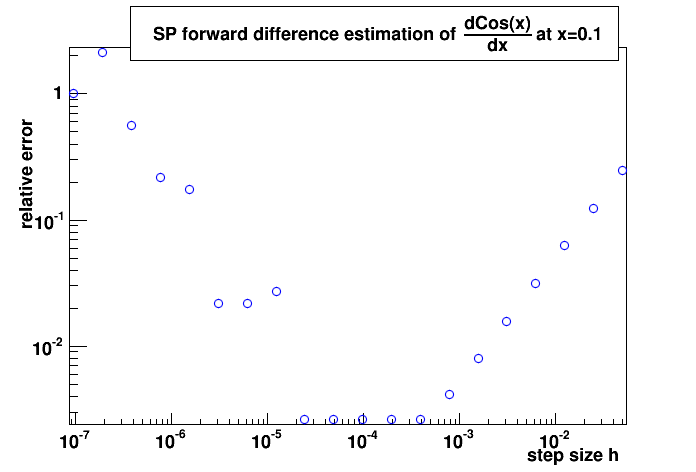
\includegraphics[scale=0.6]{cos_forward_10} 
\caption{ derivative of cosx}
\label{sat}
\end{figure}

\begin{figure}
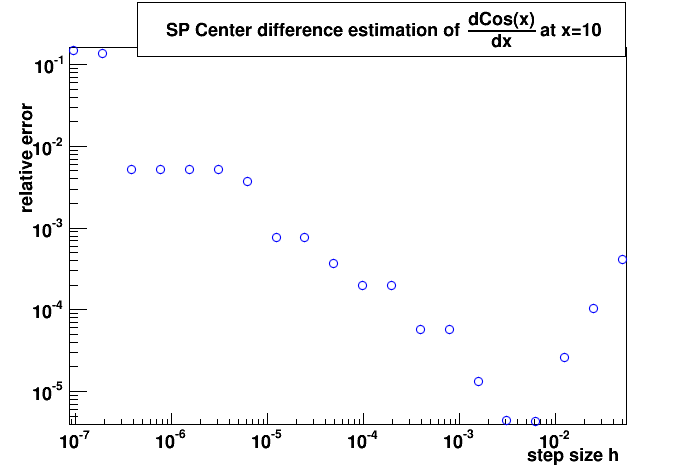
\includegraphics[scale=0.6]{cos_center_10} 
\caption{ derivative of cosx}
\label{sat}
\end{figure}

\begin{figure}
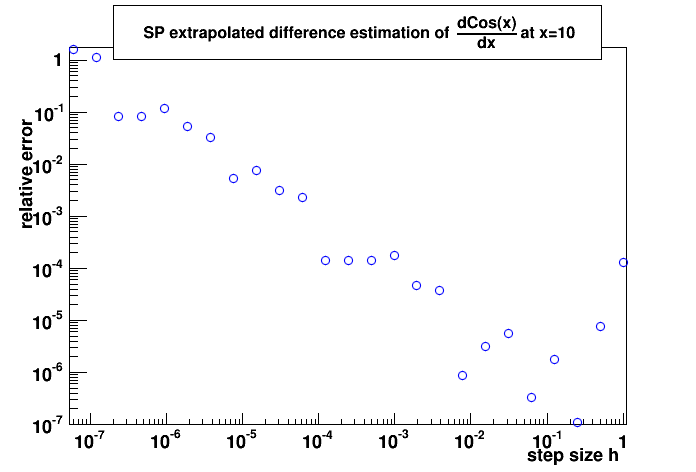
\includegraphics[scale=0.6]{cos_extra_10} 
\caption{ derivative of cosx}
\label{sat}
\end{figure}

\begin{figure}
\includegraphics[scale=0.6]{cos_exp_10} 
\caption{ derivative of cosx}
\label{sat}
\end{figure}

\begin{figure}
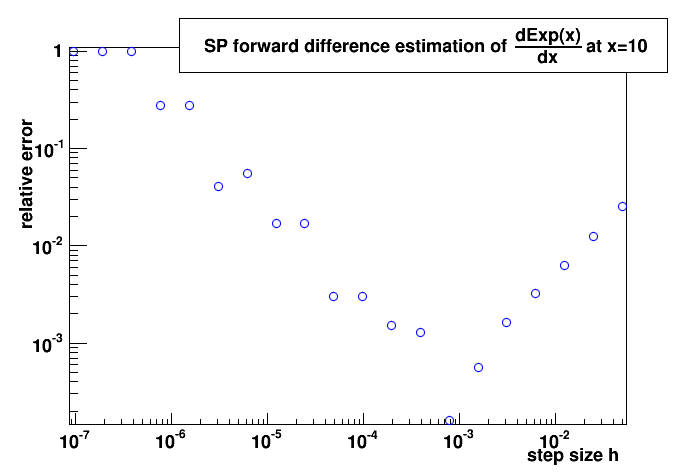
\includegraphics[scale=0.6]{exp_forward_10} 
\caption{ derivative of exp x}
\label{sat}
\end{figure}

\begin{figure}
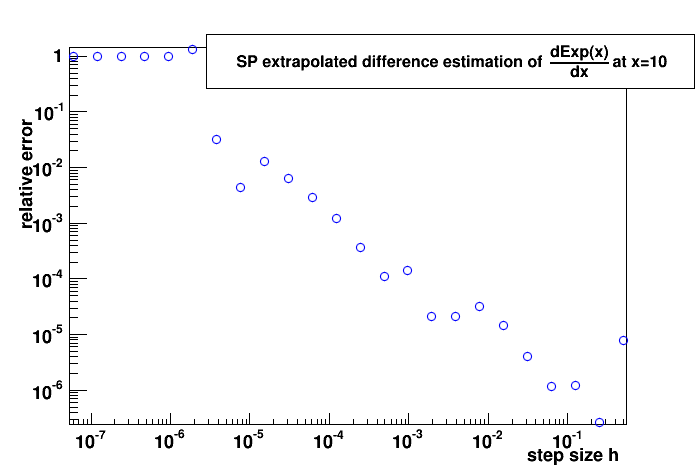
\includegraphics[scale=0.6]{exp_extra_10} 
\caption{ derivative of exp x}
\label{sat}
\end{figure}

\section{problem 2}

\begin{figure}
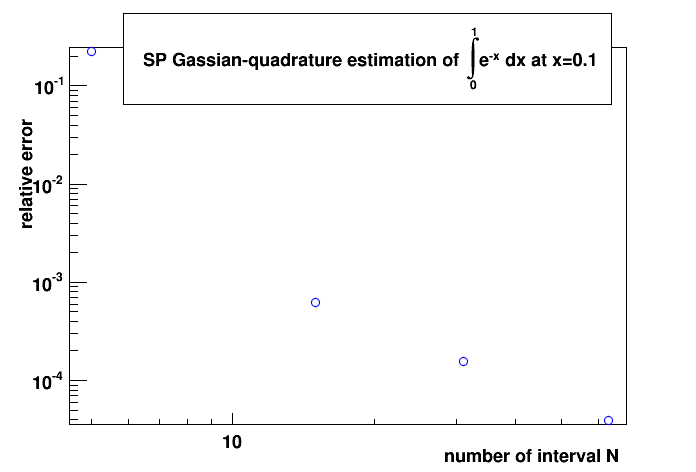
\includegraphics[scale=0.6]{2_gaussian} 
\caption{ derivative of exp x. The error is expected to be smaller for the range of N. }
\label{sat}
\end{figure}

\begin{figure}
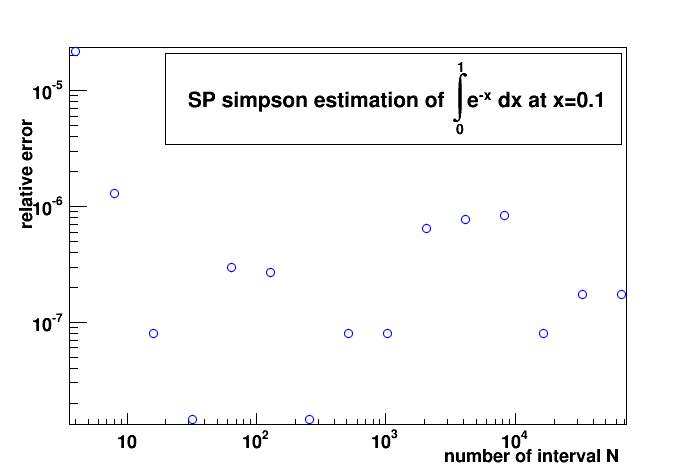
\includegraphics[scale=0.6]{2_simpson} 
\caption{ derivative of exp x}
\label{sat}
\end{figure}

\begin{figure}
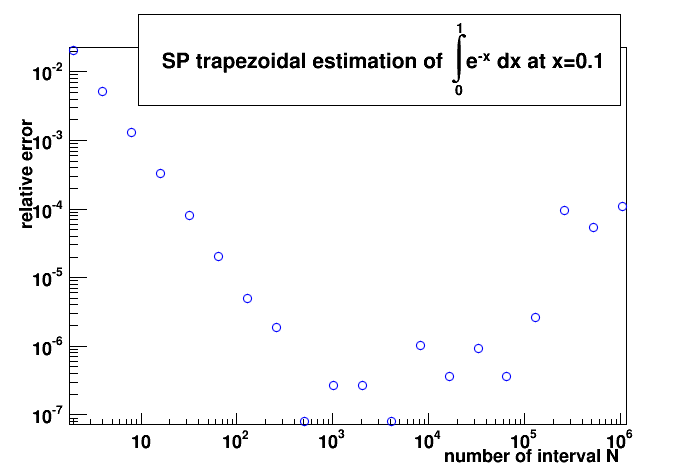
\includegraphics[scale=0.6]{2_trapezoid} 
\caption{ derivative of exp x}
\label{sat}
\end{figure}




\section{problem 3}

\begin{figure}
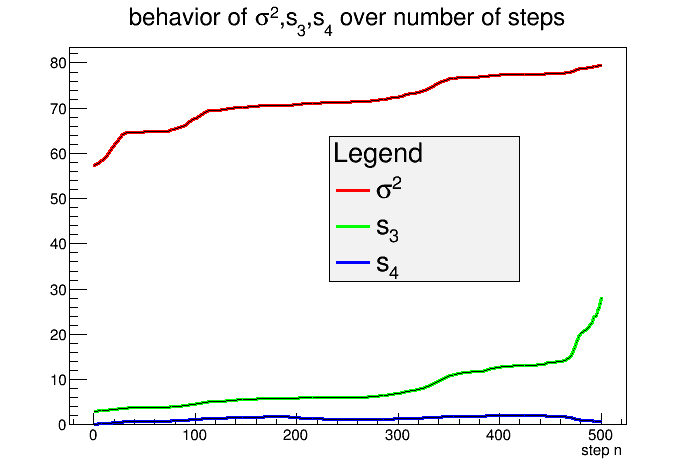
\includegraphics[scale=0.6]{3_3plots} 
\caption{ behavior plot}
\label{sat}
\end{figure}


\end{document}
%
% ****** End of file aipsamp.tex ******
